\documentclass[conference]{IEEEtran}
\IEEEoverridecommandlockouts

\usepackage{amsmath}
\usepackage{booktabs}
\usepackage{graphicx}
\usepackage{url}

% IEEEtran normally inserts an em dash after these labels. Use a plain colon
% so the paper follows the project's no-em-dash style rule.
\makeatletter
\def\abstract{\normalfont
    \if@twocolumn
      \@IEEEabskeysecsize\bfseries\textit{\abstractname:}\ \relax
    \else
      \bgroup\par\addvspace{0.5\baselineskip}\centering\vspace{-1.78ex}\@IEEEabskeysecsize\textbf{\abstractname}\par\addvspace{0.5\baselineskip}\egroup\quotation\@IEEEabskeysecsize
    \fi\@IEEEgobbleleadPARNLSP}
\def\IEEEkeywords{\normalfont
    \if@twocolumn
      \@IEEEabskeysecsize\bfseries\textit{\IEEEkeywordsname:}\ \relax
    \else
      \bgroup\par\addvspace{0.5\baselineskip}\centering\@IEEEabskeysecsize\textbf{\IEEEkeywordsname}\par\addvspace{0.5\baselineskip}\egroup\quotation\@IEEEabskeysecsize
    \fi\@IEEEgobbleleadPARNLSP}
\makeatother

\title{Auditing a Normal-First Skeleton JEPA for Monocular Gait Representations}

\author{
\IEEEauthorblockN{Theodore Mui, Alex Mui, Penny Inouye, and Phil Mui}
\IEEEauthorblockA{\textit{Aspiring Scholars Directed Research Program (ASDRP)}\\
\texttt{tedmui@stanford.edu} \quad \texttt{alexander.mui@students.asdrp.org}\\
\texttt{pennypenelopesf@gmail.com} \quad \texttt{phil.mui@asdrp.org}}
}

\begin{document}
\maketitle

\begin{abstract}
We trained and audited a skeletal Joint-Embedding Predictive Architecture, or S-JEPA, for monocular gait video. The completed normal-first curriculum used 159 pose sequences from 35 source videos. Final feature spread remained nonzero, but the normal reference representation drifted as four gait groups entered. On the canonical 96-sequence GAVD cohort, minimum cosine distance between condition centroids was 0.037, mean within-condition distance was 0.120, and cosine silhouette was 0.009. These values do not show clean five-group geometry. A stratified sequence split produced 0.793 five-class accuracy, but every test video also appeared in classifier training and every test row had already been seen by the label-aware encoder. Classifier-video-grouped folds produced mean accuracy of 0.849 for normal versus abnormal and 0.653 for five classes, but the encoder still saw all evaluation rows. The run completed without total representation collapse. It does not establish generalization to unseen videos, patients, or clinics.
\end{abstract}

\begin{IEEEkeywords}
gait analysis, joint-embedding predictive architecture, S-JEPA, VICReg, pose estimation, curriculum learning
\end{IEEEkeywords}

\section{Introduction}
Walking depends on the nervous system, muscles, joints, balance, and the surrounding environment. Parkinson's disease, stroke, and cerebral palsy can change gait \cite{zanardi2021parkinsons,lauziere2014stroke,pandey2023crouch}. Late-onset Pompe disease, one type of myopathy, can reduce motor function \cite{maulet2023myopathy}. A gait video alone cannot establish a diagnosis.

A Joint-Embedding Predictive Architecture, or JEPA, predicts hidden content in representation space rather than reconstructing every input value. This principle has been studied in images, video, and skeleton sequences \cite{assran2023ijepa,bardes2024vjepa,abdelfattah2024sjepa}. A second problem is representation collapse, where many inputs map to nearly the same vector. VICReg discourages this failure by preserving variation and reducing redundant feature dimensions \cite{bardes2022vicreg}.

We ask whether one model can first learn normal gait, continue through four broader gait groups, and retain a useful, nonconstant representation. We answer with a completed five-stage run, geometry measurements, a detector-missingness control, and exposure audits. Our contributions are a reproducible 12-landmark target rule, a continuing 159-sequence curriculum, separate measurements of collapse and normal-reference drift, and downstream scores reported with their source-video overlap.

\section{Related Work}
S-JEPA uses an exponential-moving-average teacher and a predictor for skeleton action recognition \cite{abdelfattah2024sjepa}. MAMP predicts motion and uses motion-aware target selection \cite{mao2023mamp}, while Skeleton2vec uses contextualized targets \cite{xu2024skeleton2vec}. This project uses neither target selector. It samples only from a fixed anatomical whitelist. GaitForeMer uses self-supervised forecasting for gait impairment estimation \cite{endo2022gaitforemer}. Our narrower aim is to audit a small representation-learning workflow, not to predict diagnosis or severity.

\section{Materials and Methods}
\subsection{Data and pose processing}
The canonical cohort contains 96 sequences from 18 GAVD source videos \cite{ranjan2025gavd}. The completed run also uses 63 normal sequences from 17 user-supplied videos. These added clips were selected and labeled as normal within this project. Automatic MediaPipe detections supplied their person boxes. They are not part of GAVD and did not receive independent clinical label review.

\begin{table}[t]
\caption{Representation-training corpus}
\label{tab:cohort}
\centering
\scriptsize
\begin{tabular}{lrr}
\toprule
Group & Sequences & Videos \\
\midrule
Canonical normal & 12 & 1 \\
Added normal & 63 & 17 \\
Parkinson's disease & 9 & 2 \\
Stroke & 12 & 3 \\
Myopathic & 47 & 10 \\
Cerebral palsy & 16 & 2 \\
\midrule
Total & 159 & 35 \\
\bottomrule
\end{tabular}
\end{table}

GAVD boxes isolate the intended walker. MediaPipe estimates 33 landmarks and visibility \cite{grishchenko2022blazepose,mediapipePoseLandmarker}. The pipeline uses image-relative pose estimates. Monocular depth is not calibrated clinical motion capture. Internal low-visibility gaps of at most four frames are interpolated; longer gaps stay missing. Each sequence is pelvis-centered, body-scale normalized, and resized to 64 frames. Missing coordinates cannot become prediction targets.

\subsection{Targets, model, and loss}
The sole target-rule source is \path{experiments/multiple-sclerosis/mapping-data/ms-pd-mapping.md}. It expands ranges and removes duplicates to produce
\begin{equation}
\{11,12,23,24,25,26,27,28,29,30,31,32\}.
\end{equation}
These are the left and right shoulders, hips, knees, ankles, heels, and foot indices. Reusing this whitelist across five folders is a project rule, not a diagnostic claim.

A token holds one landmark over four frames, so a sequence contains 528 tokens. The configured 0.60 fraction is applied to the smallest valid eligible-token count in each batch, and that common number is sampled uniformly without replacement in every sample. Samples with more valid tokens therefore realize a lower fraction. The sampler never reads motion. Invalid allowed tokens are skipped and forbidden landmarks are never substituted. The target encoder can still use all 33 landmarks as context.

The view encoder reads a masked pose. The target encoder reads the complete pose and follows the view encoder by exponential moving average. The predictor estimates target latents at hidden locations. The full loss is
\begin{equation}
\mathcal L=\mathcal L_{\mathrm{JEPA}}+0.05\mathcal L_{\mathrm{VICReg}}+0.25\mathcal L_{\mathrm{group}}.
\end{equation}
VICReg combines invariance, variance-hinge, and covariance terms \cite{bardes2022vicreg}. It discourages collapse but does not know folder names. The separate group term is label-aware: it encourages within-folder compactness and penalizes centroid distances below 1.0. It is zero in Stage 0.

\subsection{Continuing curriculum and audit design}
One model continues through all stages. The view encoder, predictor, target encoder, target center, and VICReg projector are never reinitialized. Later batches balance all active groups, so earlier groups remain in training.

\begin{table}[t]
\caption{Five-stage continuing curriculum}
\label{tab:curriculum}
\centering
\small
\begin{tabular}{clrr}
\toprule
Stage & Added data & Epochs & Updates \\
\midrule
0 & 75 normal & 300 & 5,700 \\
1 & 9 Parkinson's & 75 & 1,425 \\
2 & 12 stroke & 75 & 1,425 \\
3 & 47 myopathic & 75 & 1,425 \\
4 & 16 cerebral palsy & 75 & 1,425 \\
\midrule
Total & & 600 & 11,400 \\
\bottomrule
\end{tabular}
\end{table}

The final checkpoint is \path{sjepa_curriculum_final_augmented.pt}; its fingerprint begins \texttt{d0acc2628d134959}. The contract records sequence and video identifiers, stage lineage, loss settings, target-mask hash, and optimizer counts.

Figure~\ref{fig:design} summarizes the corpus and the claim boundary. We audit training health, canonical five-group geometry, and downstream Random Forest readouts \cite{breiman2001randomforests,pedregosa2011scikit}. The all-96 lane is stratified by row: normal is split 8/4, Parkinson's 6/3, stroke 9/3, myopathic 33/14, and cerebral palsy 11/5. Stratification preserves proportions but does not separate source videos. Balanced accuracy averages recall over classes \cite{brodersen2010balanced}.

The exact-47/21 lane reproduces a historical split. Lane C uses five GroupKFold splits for the binary task and two StratifiedGroupKFold splits for the five-class task. Two is the largest fold count that keeps every label on both sides because Parkinson's disease and cerebral palsy each have only two videos. A source video cannot appear in both Random Forest portions of one fold. Grouping matters when rows share a source \cite{roberts2017crossvalidation}. In all lanes, however, the encoder was trained first on the full corpus. Lane C separates videos only for the Random Forest, not for representation learning.

\begin{figure*}[t]
\centering
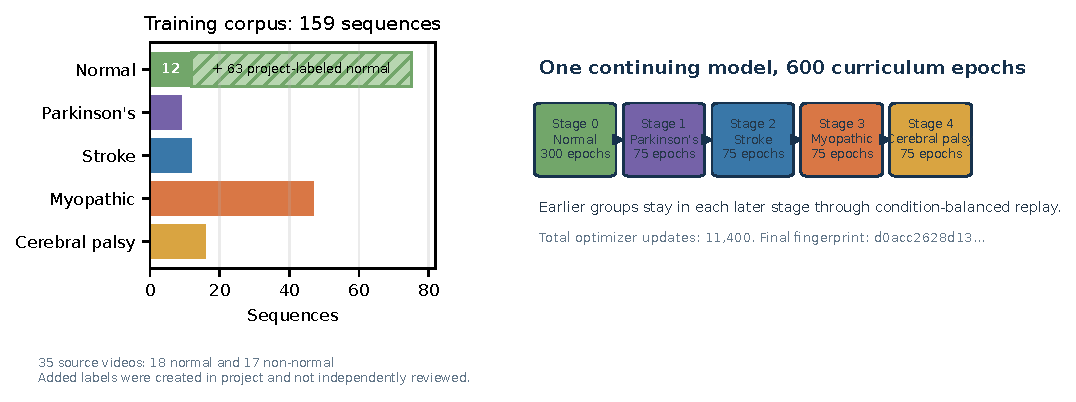
\includegraphics[width=0.495\textwidth]{figures/cohort_curriculum.pdf}\hfill
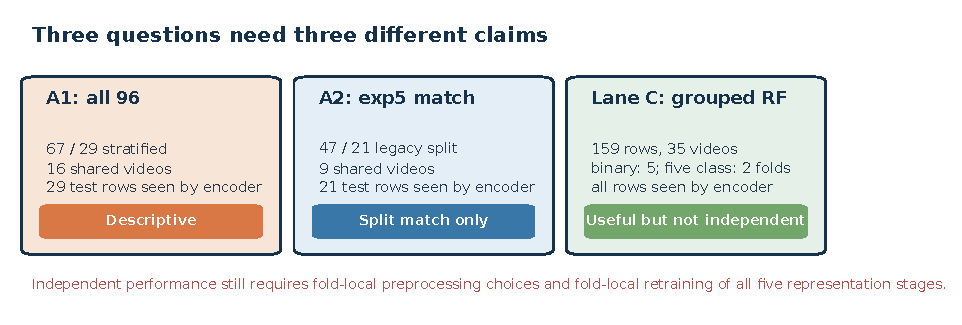
\includegraphics[width=0.495\textwidth]{figures/evidence_ladder.pdf}
\caption{Left: the 159-sequence corpus and five continuing stages. Right: each downstream lane supports a limited claim because the encoder saw its evaluation rows.}
\label{fig:design}
\end{figure*}

\section{Results}
\subsection{Training health}
The recommended run completed 600 epochs and 11,400 updates. Table~\ref{tab:health} and the left side of Fig.~\ref{fig:health_geometry} show the stage endpoints. Final feature standard deviation was 0.414 and mean pairwise cosine was 0.609. These values argue against the extreme case where every sequence has one identical representation. They do not prove that each feature is useful.

Normal-anchor cosine fell from 0.954 after Stage 1 to 0.594 after Stage 4. The model kept nonzero spread, but its normal reference changed substantially. The nonzero final margin penalty also shows that the requested training-corpus margin was not fully satisfied.

\begin{table*}[t]
\caption{Stage-end training diagnostics. The centroid values are active-corpus training diagnostics, not the separate canonical audit.}
\label{tab:health}
\centering
\small
\begin{tabular}{crrrrrr}
\toprule
Stage & JEPA loss & VICReg loss & Feature std. & Pair cosine & Min. centroid distance & Normal-anchor cosine \\
\midrule
0 & 0.569 & 16.997 & 0.466 & 0.359 & not defined & not defined \\
1 & 0.449 & 12.989 & 0.430 & 0.492 & 0.740 & 0.954 \\
2 & 0.613 & 10.474 & 0.399 & 0.624 & 0.527 & 0.839 \\
3 & 0.611 & 9.368 & 0.406 & 0.628 & 0.336 & 0.707 \\
4 & 0.478 & 8.418 & 0.414 & 0.609 & 0.364 & 0.594 \\
\bottomrule
\end{tabular}
\end{table*}

\subsection{Canonical geometry}
The frozen target encoder produced a $96\times384$ matrix for the canonical GAVD rows. Mean within-condition cosine distance was 0.120. Mean distance between centroids was 0.292, but the minimum was 0.037, between myopathic and cerebral-palsy rows. Cosine silhouette was 0.009. The weak pair is closer than the average spread within a condition, so the rows do not form five clean clusters.

The Stage 4 minimum centroid value of 0.364 in Table~\ref{tab:health} is not contradictory. It is an active-corpus training measurement over 159 rows. The right side of Fig.~\ref{fig:health_geometry} is a separate frozen target-encoder audit over the canonical 96 rows.

\begin{figure*}[t]
\centering

\includegraphics[width=0.655\textwidth]{figures/training_health.pdf}\hfill
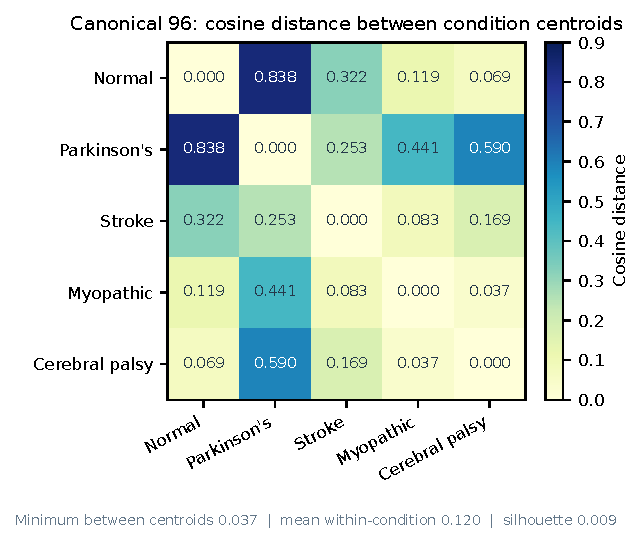
\includegraphics[width=0.325\textwidth]{figures/representation_geometry.pdf}
\caption{Left: loss and representation health across the completed curriculum. Spread stays nonzero while the normal reference drifts. Right: canonical centroid distances. Myopathic and cerebral-palsy centroids are only 0.037 apart.}
\label{fig:health_geometry}
\end{figure*}

\subsection{Downstream readouts}
Table~\ref{tab:readouts} reports descriptive readouts. The all-96 S-JEPA result exceeded the missingness-only control, but both used the same confounded split. All 16 test videos also appeared in classifier training, and all 29 test rows participated in label-aware representation training.

For Lane C normal versus abnormal, mean ROC AUC was 0.966. A percentile bootstrap over the five fold scores gave an accuracy interval of 0.800 to 0.906. This is a descriptive summary of five dependent folds, not a strong population confidence interval. The corrected five-class lane uses only two folds and reports no interval. Its pooled out-of-fold accuracy was 0.654 and pooled macro-F1 was 0.619. Ordinary K-fold cross-validation has no generally unbiased variance estimator \cite{bengio2004variance}.

\begin{table*}[t]
\caption{Descriptive downstream results. BA is balanced accuracy. Every S-JEPA evaluation row was seen during representation training.}
\label{tab:readouts}
\centering
\scriptsize
\begin{tabular}{lrrrl}
\toprule
Lane and task & Accuracy & BA & Macro F1 & Main exposure \\
\midrule
All-96 missingness control & 0.448 & 0.466 & 0.429 & 16 shared test videos \\
All-96 S-JEPA & 0.793 & 0.889 & 0.821 & 16 shared videos; 29/29 test rows seen by encoder \\
Exact-47/21 S-JEPA & 0.714 & 0.730 & 0.742 & 9 shared videos; 21/21 test rows seen by encoder \\
Historical 82-feature reference & 0.762 & not recorded & 0.728 & same confounded 47/21 split \\
Lane C normal vs. abnormal & 0.849 & 0.874 & 0.826 & grouped RF; all 159 rows seen by encoder \\
Lane C five class & 0.653 & 0.603 & 0.625 & two grouped RF folds; all 159 rows seen by encoder \\
\bottomrule
\end{tabular}
\end{table*}

\begin{figure*}[t]
\centering
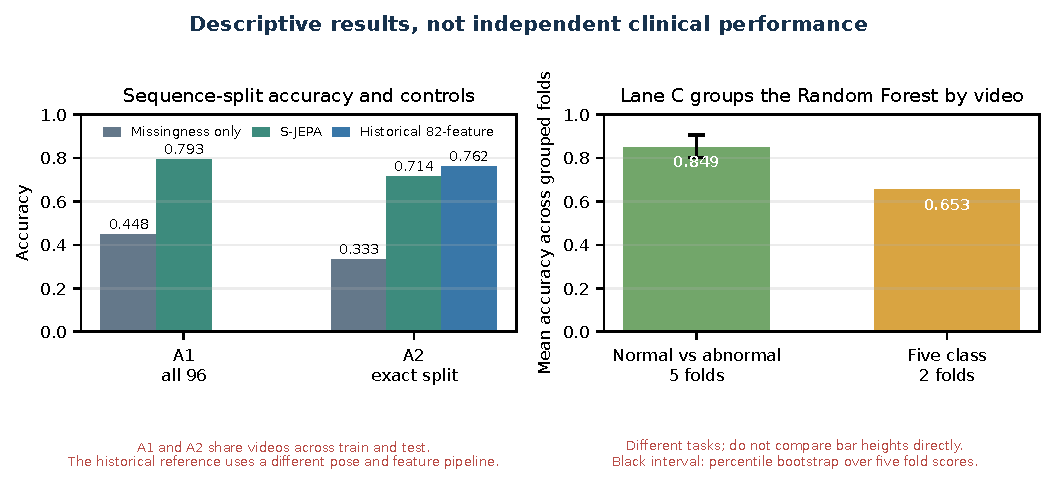
\includegraphics[width=0.86\textwidth]{figures/readout_results.pdf}
\caption{Accuracy across the current readout lanes. The black interval belongs only to the five-fold binary Lane C task. The corrected two-fold five-class task intentionally has no interval. Every score remains descriptive because the encoder saw its evaluation rows.}
\label{fig:readout_results}
\end{figure*}

\section{Discussion}
The run answers the implementation question. One model continued through all five stages, checkpoints preserved lineage, the target whitelist stayed intact, and feature spread did not vanish. It also reveals two weaknesses. First, a final normal-anchor cosine of 0.594 shows substantial drift despite balanced replay. Second, a canonical silhouette of 0.009 and minimum centroid distance below within-condition spread do not support a claim of five separated gait groups.

A Random Forest can still draw nonlinear boundaries, especially when video identity, pose-detector behavior, or label-aware representation training supplies extra signals. The missingness control reaching 0.448 accuracy shows that detector behavior contains condition-related information, although it does not explain the full S-JEPA score.

The data structure prevents stronger conclusions. All 12 canonical normal rows come from one video. Parkinson's disease and cerebral palsy each have only two videos. This limits the corrected five-class grouped audit to two folds, which is too little support for a stable performance claim. The 63 added normal rows improve video variety, but their labels were produced inside this project and were not independently reviewed.

An independent estimate needs a nested experiment. Each outer source-video fold must choose and freeze preprocessing rules, train all five representation stages, and fit the Random Forest using only training videos. Held-out videos must remain unseen until final scoring. More independent people, sites, camera setups, and clinical label review are also needed.

\section{Conclusion}
The full normal-first S-JEPA curriculum trained on 159 sequences without complete representation collapse. It did not preserve the normal reference well, and the canonical rows did not form clean five-condition geometry. Current classifier results are descriptive because source videos, representation-training rows, or both overlap evaluation. The workflow is auditable and its weaknesses are measurable, but it is not yet evidence of clinical usefulness or unseen-video generalization.

\IEEEtriggeratref{16}
\bibliographystyle{IEEEtran}
\bibliography{references}

\end{document}
